\title{ТР №4 Муртазин Рифат}
\date{May 2020}
\documentclass[a4paper]{article}
\usepackage{booktabs}
\usepackage{array,graphicx,caption}
\usepackage{graphicx}
\usepackage[rightcaption]{sidecap}
\usepackage{wrapfig}
\usepackage[14pt]{extsizes} % для того чтобы задать нестандартный 14-ый размер шрифта
\usepackage[utf8x]{inputenc}
\usepackage[table,xcdraw]{xcolor}
\usepackage[russian]{babel}
\usepackage{setspace,amsmath}
\usepackage{amssymb}
\usepackage{graphicx}
\graphicspath{ {./images/} }
\usepackage[left=20mm, top=15mm, right=15mm, bottom=15mm, nohead, footskip=10mm]{geometry} % настройки полей документа
\begin{document} % начало документа
 
% НАЧАЛО ТИТУЛЬНОГО ЛИСТА
\begin{center}
\hfill \break
\large{МИНИСТЕРСТВО НАУКИ И ВЫСШЕГО ОБРАЗОВАНИЯ РОССИЙСКОЙ ФЕДЕРАЦИИ}\\
\footnotesize{федеральное государственное автономное образовательное учреждение высшего образования}\\ 
\small{\textbf{«Санкт-Петербургский национальный исследовательский университет информационных технологий, механики и оптики»}}\\
\hfill \break
\normalsize{Мегафакультет трансляционных информационных технологий}\\
 \hfill \break
\normalsize{Факультет информационных технологий и программирования}\\
\hfill\break
\hfill \break
\hfill \break
\hfill \break
\large{\Huge{Типовой расчёт №4}}\\
\Large{По дисциплине “Дискретная математика”}\\
\Large{По теме «Теория графов и комбинаторика»}\\
\hfill \break
\hfill \break

\hfill \break

\hfill \break
\large{ \hspace{28pt} Выполнил студент группы №M3112} \hfill \break
\large{ \hspace{28pt} Муртазин Рифат Фаритович} \hfill \break
\hfill \break
\large{ \hspace{28pt} Проверил} \hfill \break
\large{ \hspace{28pt} Кочетков Никита} \hfill \break
\hfill \break
\hfill \break
\hfill \break
\hfill \break
\begin{center} Санкт-Петербург 2020 \end{center}
\thispagestyle{empty} % выключаем отображение номера для этой страницы
 
% КОНЕЦ ТИТУЛЬНОГО ЛИСТА

\newpage
 
\newpage

\section{задание}

\begin{flushleft}
    \textbf{{\Large Условие}}
\end{flushleft}
(1 балл) На книжной полке стоят 12 книг. Сколькими способами можно вытащить 5 из них так, чтобы никакие две из них не стояли рядом?
\hfill \break

\begin{flushleft}
    \textbf{{\Large Решение}}
\end{flushleft}

\begin{flushleft}
    Данную задачу можно решить с помощью формулы сочетания без повторений, потому что нам не важен порядок в выборке. \textbf{Сочетание} - это неупорядоченный набор размера n из m элементов \[C(n, m)=C_m^n=\frac{m!}{(m - n)!*n!}\]
    Можно заметить что \[\frac{m!}{(m - n)!}\] - это формула размещения.
    Получается, что в сочетаниях мы вначале всё размещаем, а потом делим всё на все возможные перестановки - n!, \textbf{чтобы избавиться от всех возможных перестановок и оставить только один набор}. Следовательно, возвращаясь к задаче, нам нужно убрать 5 книг или сочетать 5 объектов, то есть n = 5. Мы можем их убрать в 8-ми местах, так как можно убрать каждую через один пропуск - это 6 мест и 2 места по краям. Таким образом получаем 8 элементов, которые осталось сочетать по 5-ть. Остаётся подставить в формулу сочетаний. Получаем \[C_8^5=\frac{8!}{(8 - 5)!*5!}=\frac{40320}{6*120}=56\]
    \textbf{Ответ: 56.}
\end{flushleft}

\newpage

\section{задание}

\begin{flushleft}
    \textbf{{\Large Условие}}
\end{flushleft}
(1 балл) Я хочу послать своему другу 8 фотографий. Сколькими способами я могу разложить их по 5-ти конвертам?
\hfill \break

\begin{flushleft}
    \textbf{{\Large Решение}}
\end{flushleft}

\begin{flushleft}
    Для того чтобы решить эту задачу, нужно воспользовать формулой включений-исключений \begin{gather*} \sum_{i} | A_i | - \sum_{i<j} | A_i \cap A_j | + \sum_{i<j<k} | A_i \cap A_j \cap A_k | - \\ - \ldots + (-1)^{n-1} | A_1 \cap A_2 \cap \ldots \cap A_n | \end{gather*}
    адаптируем формулу под нашу задачу и получим:
    \begin{gather*} m^{n} - C_m^1(m - 1)^{n}+C_m^2(m - 2)^{n}-\ldots+
    (-1)^{k}*C_m^k(m - k)^{n}+\ldots+ \\ +(-1)^{m-1}C_n^{m - 1} \end{gather*}
    пусть n = 8, а m = 5. Тогда подставим в формулу.
    \begin{gather*} 5^8 - C_5^1*(5-1)^8+C_5^2*(5-2)^8 -C_5^3*(5-3)^8+C_5^4*(5-4)^8= \\ =5^8 - C_5^1*(4)^8+C_5^2*(3)^8-C_5^3*(2)^8+C_5^4*(1)^8=\\=5^8 - \frac{5!}{4!}*(4)^8+\frac{5!}{3!*2!}*(3)^8-\frac{5!}{2!*3!}*(2)^8+\frac{5!}{1!*4!}*(1)^8=\\=5^8 - 5*4^8+10*3^8-10*2^8+5=\\= 390625 - 327680 + 65610 - 2560 + 5 =126000  \end{gather*}
    \textbf{Ответ: 126000.}
\end{flushleft}

\newpage

\section{задание}

\begin{flushleft}
    \textbf{{\Large Условие}}
\end{flushleft}
\begin{flushleft}
(1 балл) Пирамидка, в которую играет ребенок, состоит из 49 дисков, по 7 каждого размера (диски од- ного размера неразличимы). Пирамидка устроена таким образом, что на нижнем слое может находиться только самый большой диск, а на верхнем слое только самый маленький. Мы будем называть правильной сборкой пирамидки такую последовательность из семи дисков, что каждый следующий не больше предыдущего, первый диск будет самого большого размера, а последний − самого маленького (например, 7654321, 7775331, и 7222211 являются правильными сборками, а 7654322 − не правильной). Сколько всего существует правильных сборок?
\end{flushleft}
\hfill \break

\begin{flushleft}
    \textbf{{\Large Решение}}
\end{flushleft}
\begin{flushleft}
    Решается эта задача с помощью сочетания. Учтём тот факт, что у нас в условии сказано, что "Пирамидка устроена таким образом, что на нижнем слое может находиться только самый большой диск, а на верхнем слое только самый маленький", следовательно у двух дисков уже определены позиции - это первая и последняя. Учтём также, что по условию могут идти подрят одиноковые по размеру диски, тогда можно сделать вывод, что у нас в сочетаниях есть повторения, тогда следует использовать готовую формулу сочетания с повторениями:
    \begin{gather*}\tilde{\sf C}_n^k={(n+k-1)!\over k!(n-1)!}={\sf C}_{n+k-1}^k.\end{gather*}
    В нашем случаи $k = 5$, потому что две позиции уже заняты, $n = 7$.
    Подставим в уравнение значения и посчитаем:
    \begin{gather*}\tilde{\sf C}_n^k={(n+k-1)!\over k!(n-1)!}=\\={(7+5-1)!\over 5!(7-1)!}={11!\over 5!6!}={39916800\over 86400}=462.\end{gather*}
    \textbf{Ответ: 462.}
\end{flushleft}

\section{задание}

\begin{flushleft}
    \textbf{{\Large Условие}}
\end{flushleft}
(1 балл) В стране 20 городов, каждые два из которых соединены авиалинией. Сколько авиалиний в этой стране?
\hfill \break

\begin{flushleft}
    \textbf{{\Large Решение}}
\end{flushleft}

\begin{flushleft}
    Решение основано на принципе умножения, потому что применим, когда у нас есть, какое то множество событий, которое происходит последовательно или события, которые осуществляются вне зависимости друг от друга. У нас есть два города, которые имеют общую авиалинию, но в стране всего 20 городов. Для выбора первого есть 20 городов, для выбора второго такого города остаётся 19. Следовательно перемножаем 19 и 20, а потом делим результат на 2, потому что авиалиния обща для двух городов. Имеем: ${20*19\over 2}={190}$.
    \textbf{Ответ: 190.}
\end{flushleft}

\newpage

\section{задание}

\begin{flushleft}
    \textbf{{\Large Условие}}
\end{flushleft}
\begin{flushleft}
(2 балла) Для представленного графа определите:
\begin{figure}[h]
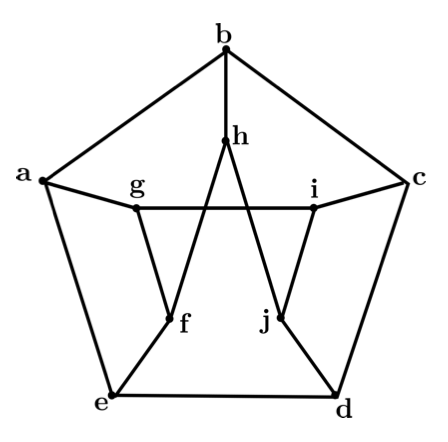
\includegraphics[scale=1.2]{graph}
\centering
\end{figure}
\begin{enumerate}
  \item есть ли в графе Эйлеров цикл или Эйлерова цепь? Если есть, то выпишите. Если нет, то обоснуйте отсутствие;
  \item есть ли в графе Гамильтонов цикл, Гамильтонова цепь? Если есть, то выпишите. Если нет, то обоснуйте отсут- ствие;
\end{enumerate}
\end{flushleft}
\hfill \break
\begin{flushleft}
    \textbf{{\Large Решение}}
\end{flushleft}
\begin{flushleft}
\begin{enumerate}
  \item\textbf{Эйлеровой цепью} в графе называется путь, который проходит по каждому       ребру, причем ровно один раз.
        \textbf{Эйлеров цикл} — замкнутый эйлеров путь.
        В данном графе нет \textbf{Эйлеровой цепи} и \textbf{Эйлерового цикла}, потому что отсутсвует такой путь, который проходит по каждому ребру один раз. Граф так же не Эйлеров,так как количество вершин с нечетной степенью больше дву. Если количество вершин с нечетной степенью больше двух, то граф не является Эйлеровым\textbf{Следователь граф не содержит Эйлеров цикл и Эйлеров путь и соответственно не Эйлеров}.
  \item \textbf{Гамильтоновым путём} называется простой путь, проходящий через каждую вершину графа ровно один раз. \textbf{Гамильтоновым циклом} называют замкнутый гамильтонов путь. \textbf{Данный граф содержит Гамильтонов путь, проходящий по a => b => c => d => e => f => g => i => j => h. Данный граф содержит Гамильтонов цикл, проходящий по a => b => c => d => e => f => h => j => i => g => a}.
\end{enumerate}
\end{flushleft}

\newpage

\section{задание}

\begin{flushleft}
    \textbf{{\Large Условие}}
\end{flushleft}
\begin{flushleft}
(1 балл) Нарисуйте графы К6 и К3,4, К 7,5.
\end{flushleft}
\hfill \break

\begin{flushleft}
    \textbf{{\Large Решение}}
\end{flushleft}
\begin{flushleft}
    Простой граф с $n$ взаимными вершинами обозначается {\Large$K_n$}. Граф, в котором каждая пара различных вершин смежна \textbf{называется полным}. Полный граф с $n$ вершинами имеет $n(n-1) \over 2$ рёбер.
    \textbf{Двудольный граф} — граф, множество вершин которого можно разбить на две части таким образом, что каждое ребро графа соединяет какую-то вершину из одной части с какой-то вершиной другой части, то есть не существует ребра, соединяющего две вершины из одной и той же части. Двудольный граф с $n$ вершинами в одной доле и $m$ во второй обозначается {\Large$K_{n,m}$}.
    \begin{figure}[h]
    \centering
    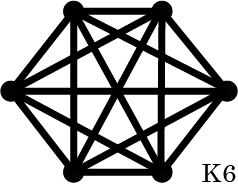
\includegraphics[width=0.5\textwidth]{k6}
    \caption{Полный граф с 6-ю вершинами - $K_6$}
    \label{fig:graph}
    \end{figure}
    \begin{figure}[!]
    \centering
    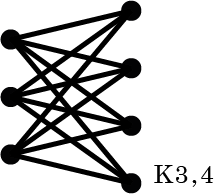
\includegraphics[width=0.5\textwidth]{k34}
    \caption{Двудольный граф с 7-ю вершинами}
    \label{fig:graph}
    \end{figure}
    \begin{figure}[!]
    \centering
    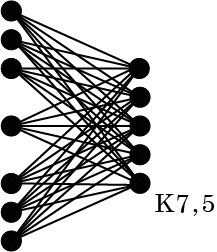
\includegraphics[width=0.5\textwidth]{k75}
    \caption{Двудольный граф с 12-ю вершинами}
    \label{fig:graph}
    \end{figure}
\end{flushleft}

\newpage
\newpage

\section{задание}

\begin{flushleft}
    \textbf{{\Large Условие}}
\end{flushleft}
\begin{flushleft}
(3 балла) Граф задан матрицей расстояний. Требуется:
\begin{figure}[h]
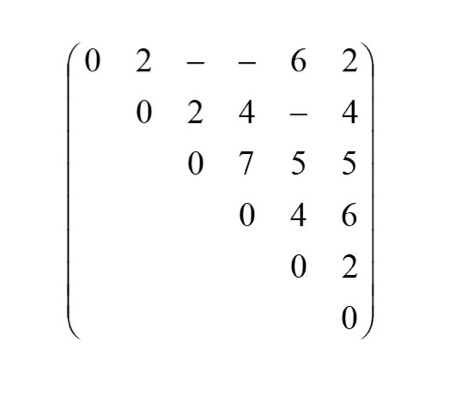
\includegraphics[scale=1.2]{matrix}
\centering
\end{figure}
\begin{enumerate}
  \item построить минимальное остовное дерево;
  \item построить фундаментальную систему циклов, ассоциированную с этим остовом;
  \item найти кратчайшие пути от вершины 4 до всех остальных вершин графа.
\end{enumerate}
\end{flushleft}
\hfill
\begin{flushleft}
    \textbf{{\Large Решение}}
\end{flushleft}
\begin{flushleft}
    Изобразим граф по матрице расстояний. Получим:
    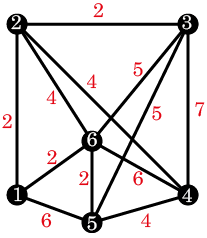
\includegraphics[scale=0.7]{images/lastgraph.png}
    1.
    \textbf{Минимальное остовное дерево графа} $G=(V,E)$— это его ациклический связный подграф, в который входят все его вершины, обладающий минимальным суммарным весом ребер.
    Для его нахождения можно использовать \textbf{алгоритм Прима}. Вначале на вход алгоритма подаётся связный неориентированный граф. Для каждого ребра задаётся его стоимость. Сначала берётся произвольная вершина и находится ребро, инцидентное данной вершине и обладающее наименьшей стоимостью. Найденное ребро и соединяемые им две вершины образуют дерево. Затем, рассматриваются рёбра графа, один конец которых — уже принадлежащая дереву вершина, а другой — нет; из этих рёбер выбирается ребро наименьшей стоимости. Выбираемое на каждом шаге ребро присоединяется к дереву. Рост дерева происходит до тех пор, пока не будут исчерпаны все вершины исходного графа.
    Результатом работы алгоритма является остовное дерево минимальной стоимости.
    \textbf{Пользуясь алгоритмом Прима, построим минимальное остовное дерево.
    Получим:}
    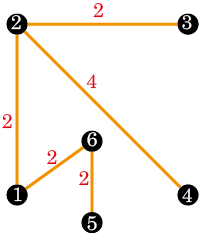
\includegraphics[scale=0.7]{images/mst.png}
    Тогда вес минимального оставного дерева $= 12$
    \textbf{Это и будет ответов на первый пункт задачи.}
\end{flushleft}
\begin{flushleft}
2.\textbf{Фундаментальный цикл графа $G$ относительно остова $T$} — простой цикл $C$, полученный путем добавления к остову $T$ ребра $e1e2∉T$.
Для того чтобы посчитать число фундаментальных циклов, нужно $m - n + 1$, где $m$ - количество рёбер в графе, $n$ - число вершин. Тогда получим $11 - 6 + 1 = 4$ \textbf{фундаментальных цикла}. Число фундаментальных циклов равно числу рёбер не пренадлежащих остову.
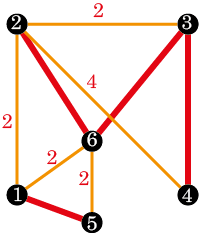
\includegraphics[scale=1]{images/cycle.png}
\end{flushleft}
\begin{flushleft}
На рисунке рёбра красного цвета образуют фундаментальные циклы и их 4 штуки, следовательно это верное количество, так как по формуле также выходит 4. Так ребро инцедентное вершинам 2 и 6 образует цикл из вершин 2, 1, 6, ребро инцедентное вершинам 3 и 6 образует цикл из вершин 2, 1, 6, 3, ребро инцедентное вершинам 3 и 4 образует цикл из вершин 3, 4, 2, ребро инцедентное вершинам 1 и 5 образует цикл из вершин 5, 1, 6.
\end{flushleft}
\begin{flushleft}
3. Чтобы найти кратчайшие пути от вершины 4 до всех остальных вершин графа, алгоритмом Дейкстры. Алгоритм работает пошагово — на каждом шаге он «посещает» одну вершину и пытается уменьшать метки. Работа алгоритма завершается, когда все вершины посещены.
Если все вершины посещены, алгоритм завершается. В противном случае, из ещё не посещённых вершин выбирается вершина u, имеющая минимальную метку. Мы рассматриваем всевозможные маршруты, в которых u является предпоследним пунктом. Вершины, в которые ведут рёбра из u, назовём соседями этой вершины. Для каждого соседа вершины u, кроме отмеченных как посещённые, рассмотрим новую длину пути, равную сумме значений текущей метки u и длины ребра, соединяющего u с этим соседом. Если полученное значение длины меньше значения метки соседа, заменим значение метки полученным значением длины. Рассмотрев всех соседей, пометим вершину u как посещённую и повторим шаг алгоритма.
\end{flushleft}
\begin{flushleft}
И так из вершины \textbf{4 в 1} кратчайший путь - \textbf{4 -> 2 -> 1} равный 6.
Из вершины \textbf{4 в 2} кратчайший путь - \textbf{4 -> 2} равный 4.
Из вершины \textbf{4 в 3} кратчайший путь - \textbf{4 -> 2 -> 3} равный 6.
Из вершины \textbf{4 в 5} кратчайший путь - \textbf{4 -> 5} равный 4.
Из вершины \textbf{4 в 6} кратчайший путь - \textbf{4 -> 6} равный 6.
В итоге получили все кратчайшие пути от вершины 4 до всех остальных вершин графа.
\end{flushleft}
\end{center}
\end{document}

